% !TEX program = pdflatex
% !TEX options = -synctex=1 -interaction=nonstopmode -file-line-error "%DOC%"
% 作业模板
\documentclass[UTF8,10pt,a4paper]{article}
\usepackage{ctex}
\newfontfamily\menlo{MONACO.TTF}
\usepackage{amsmath}
\usepackage{diagbox}
\usepackage{float}
\usepackage{listings}
\usepackage{multirow}
\usepackage{tabularx}

\usepackage{url}
\usepackage{xcolor}
\newcommand{\tabincell}[2]{\begin{tabular}{@{}#1@{}}#2\end{tabular}}

\lstset{
    breaklines,                                 % 自动将长的代码行换行排版
    extendedchars=false,                        % 解决代码跨页时,章节标题,页眉等汉字不显示的问题
    backgroundcolor=\color[rgb]{0.96,0.96,0.96},% 背景颜色
    keywordstyle=\color{blue}\bfseries,         % 关键字颜色
    identifierstyle=\color{black},              % 普通标识符颜色
    commentstyle=\color[rgb]{0,0.6,0},          % 注释颜色
    stringstyle=\color[rgb]{0.58,0,0.82},       % 字符串颜色
    showstringspaces=false,                     % 不显示字符串内的空格
    numbers=left,                               % 显示行号
    numberstyle=\tiny\menlo,                    % 设置数字字体
    basicstyle=\small\menlo,                    % 设置基本字体
    captionpos=t,                               % title在上方(在bottom即为b)
    frame=single,                               % 设置代码框形式
    rulecolor=\color[rgb]{0.8,0.8,0.8},         % 设置代码框颜色
}  

\usepackage{pythonhighlight}
\usepackage{listings}
\usepackage{xcolor}
\usepackage{graphicx}
\usepackage[a4paper,left=2cm,right=2cm,top=2cm,bottom=2cm]{geometry}
\usepackage{fancyhdr}
% \catcode`\。=\active
% \newcommand{。}{.}
\newcommand{\CourseName}{操作系统(Operating System)}
\newcommand{\CourseCode}{CS307 \& CS356}
\newcommand{\Semester}{2020-2021学年第二学期}
\newcommand{\ProjectName} {\Huge{Project 5}} 
\newcommand{\StudentName}{刘涵之}
\newcommand{\StudentID}{519021910102}
\usepackage[vmargin=1in,hmargin=.5in]{geometry}
\usepackage{fancyhdr}
\usepackage{lastpage}
\usepackage{calc}
\pagestyle{fancy}
\fancyhf{}
\fancyhead[L]{\CourseName}
\fancyhead[C]{\ProjectName}
\fancyhead[R]{\StudentName}
\fancyfoot[R]{\thepage\ / \pageref{LastPage}}
\setlength\headheight{12pt}
\fancypagestyle{FirstPageStyle}{
    \fancyhf{}
    \fancyhead[L]{\CourseName\\
        \CourseCode\\
        \Semester}
    \fancyhead[C]{\large\bfseries\ProjectName \\}
    \fancyhead[R]{Name: \makebox[\widthof{\StudentID}][s]{\StudentName}\\
        ID : \StudentID\\
        }
    \fancyfoot[R]{\thepage\ / \pageref{LastPage}}
    \setlength\headheight{36pt}
}
\usepackage{amsmath,amssymb,amsthm,bm}
\allowdisplaybreaks[4]
\newtheoremstyle{Problem}
{}
{}
{}
{}
{\bfseries}
{.}
{ }
{第\thmnumber{ #2}\thmname{ #1}\thmnote{ (#3)} 得分: \underline{\qquad\qquad}}
\theoremstyle{Problem}
\newtheorem{prob}{题}
\newtheoremstyle{Solution}
{}
{}
{}
{}
{\bfseries}
{:}
{ }
{\thmname{#1}}
\makeatletter
\def\@endtheorem{\qed\endtrivlist\@endpefalse}
\makeatother
\theoremstyle{Solution}
\newtheorem*{sol}{解}
\title{Project 5: Designing a Thread Pool & The Producer–Consumer Problem}
\date{}
% \usepackage{graphicx}
\begin{document}
\maketitle
\thispagestyle{FirstPageStyle}

\section{Designing a Thread Pool}

Thread pools were introduced in the OS book. When thread pools are used, a task is submitted to the pool and executed by a thread from the pool. Work is submitted to the pool using a queue, and an available thread removes work from the queue. If there are no available threads, the work remains queued until one becomes available. If there is no work, threads await notification until
a task becomes available.

This project involves creating and managing a thread pool, and it may be completed using either Pthreds and POSIX synchronization or Java.

In the source code download we provide the C source file \texttt{threadpool.c} as a partial implementation of the thread pool. You will need to implement the functions that are called by client users, as well as several additional functions that support the internals of the thread pool. Implementation will involve the following activities:

\begin{itemize}
    \item The \textbf{\textbf{pool\_init()}} function will create the threads at startup as well as initialize mutual-exclusion locks and semaphores.
    \item The \textbf{pool\_submit()} function is partially implemented and currently places the function to be executed—as well as its data— into a task struct. The task struct represents work that will be completed by a thread in the pool. \textbf{pool\_submit()} will add these tasks to the queue by invoking the \textbf{enqueue()} function, and worker threads will call \textbf{dequeue()} to retrieve work from the queue. The queue may be implemented statically (using arrays) or dynamically (using a linked list).

    The \textbf{pool\_init()} function has an int return value that is used to indicate if the task was successfully submitted to the pool (0 indicates success, 1 indicates failure). If the queue is implemented using arrays, \textbf{pool\_init()} will return 1 if there is an attempt to submit work and the queue is full. If the queue is implemented as a linked list, \textbf{pool\_init()} should always return 0 unless a memory allocation error occurs.
    
    \item The \textbf{worker()} function is executed by each thread in the pool, where each thread will wait for available work. Once work becomes available, the thread will remove it from the queue and invoke \textbf{execute()} to run the specified function.

    A semaphore can be used for notifying a waiting thread when work is submitted to the thread pool. Either named or unnamed semaphores may be used.
    
    \item A mutex lock is necessary to avoid race conditions when accessing or modifying the queue.
    
    \item The pool shutdown() function will cancel each worker thread and then wait for each thread to terminate by calling \textbf{pthread\_join()}. The semaphore operation \textbf{sem\_wait()} is a cancellation point that allows a thread waiting on a semaphore to be cancelled.
\end{itemize}


\newpage

\textbf{Design:} My design for this task is shown as follows:

\begin{itemize}
    \item To track all threads on the thread pool, the linked list structure \texttt{work\_queue} is implemented.
    \item A semaphore \textbf{thread\_sem} and a mutex \textbf{thread\_mut} is used to solve the critical section.
    \item A \textbf{worker} should wait the semaphore \textbf{thread\_sem}, and if \textbf{running} is equal to 1 (which means the thread pool is closed), the worker will stop its job and exit.
    \item The critical section here is the \textbf{dequeue()} function. The mutex \textbf{thread\_mut} is used to solve it.
\end{itemize}


Implementation of thread pool is shown as follows. (thread\_pool.c)
\begin{lstlisting}[language = c]
#include <pthread.h>
#include <stdlib.h>
#include <stdio.h>
#include <semaphore.h>
#include "threadpool.h"

#define QUEUE_SIZE 10
#define NUMBER_OF_THREADS 3

#define TRUE 1

// this represents work that has to be 
// completed by a thread in the pool
typedef struct
{
    void (*function)(void *p);
    void *data;
}task;

struct work_queue
{
    task work;
    struct work_queue *next;
};

// task
task task_to_do;

// the work queue
struct work_queue worktodo;
struct work_queue *head, *tail;
// the worker bee
pthread_t bee[NUMBER_OF_THREADS];

//mutex
pthread_mutex_t thread_mut;

//sem
sem_t thread_sem;

//todo or not todo
int running;

// insert a task into the queue
// returns 0 if successful or 1 otherwise, 
int enqueue(task t) 
{
    tail -> next = (struct work_queue *) malloc (sizeof (struct work_queue));
    if (tail -> next == NULL) {
        fprintf(stderr, "[Error] cannot malloc memory!\n");
		exit(1);
    }

    tail = tail -> next;
    tail -> work = t;

    return 0;
}

// remove a task from the queue
task dequeue() 
{
    if (head == tail) {
        fprintf(stderr, "[Error] No work remains!\n");
		exit(1);
    }

    head = head -> next;

    return head -> work;
}

// the worker thread in the thread pool
void *worker(void *param)
{
    while (TRUE) {
        sem_wait(&thread_sem);

        if (running == 1) break;

        pthread_mutex_lock(&thread_mut);
        task_to_do = dequeue();
        pthread_mutex_unlock(&thread_mut);

        // execute the task
        execute(task_to_do.function, task_to_do.data);
    }

    pthread_exit(0);
}

/**
 * Executes the task provided to the thread pool
 */
void execute(void (*somefunction)(void *p), void *p)
{
    (*somefunction)(p);
}

/**
 * Submits work to the pool.
 */
int pool_submit(void (*somefunction)(void *p), void *p)
{
    task_to_do.function = somefunction;
    task_to_do.data = p;
    
    pthread_mutex_lock(&thread_mut);
    int result = enqueue(task_to_do);
    pthread_mutex_unlock(&thread_mut);

    if (result == 0) {
        sem_post(&thread_sem);
    }
    return result;
}

// initialize the thread pool
void pool_init(void)
{
    running = 0;
    head = (struct work_queue *) malloc (sizeof (struct work_queue));
    if (head == NULL) {
        fprintf(stderr, "[Error] cannot malloc memory!\n");
		exit(1);
    }
    tail = head;
    head->next = NULL;

    // create mutex
    if (pthread_mutex_init(&thread_mut, NULL)){
        fprintf(stderr, "[Error] cannot create mutex!\n");
		exit(1);
    }

    // create semaphore
    if (sem_init(&thread_sem, 0, 0)) {
        fprintf(stderr, "[Error] cannot create semaphore!\n");
		exit(1);
    }

    // create threads
    for (int i = 0; i < NUMBER_OF_THREADS; i++) {
        if(pthread_create(&bee[i],NULL,worker,NULL)) {
            fprintf(stderr, "[Error] cannot create thread!\n");
			exit(1);
        }
    }

    fprintf(stdout, "[ThreadPool] Initialize successfully!\n");
}

// shutdown the thread pool
void pool_shutdown(void)
{
    running = 1;

    // set semaphore
    for (int i = 0; i < NUMBER_OF_THREADS; i++) {
        sem_post(&thread_sem);
    }

    // join
    for (int i = 0; i < NUMBER_OF_THREADS; i++) {
        if (pthread_join(bee[i],NULL)) {
            fprintf(stderr, "[Error] cannot join thread!\n");
			exit(1);
        }
    }

    // destroy
    if (pthread_mutex_destroy(&thread_mut) || sem_destroy(&thread_sem)) {
        fprintf(stderr, "[Error] cannot destroy semaphore or mutex!\n");
		exit(1);
    }

    fprintf(stdout, "[ThreadPool] Shutdown successfully!\n");
}
\end{lstlisting}



Makefile for thread-pool task is shown as follow.
\begin{lstlisting}
CC=gcc
CFLAGS=-Wall
PTHREADS=-lpthread

all: client.o threadpool.o
	$(CC) $(CFLAGS) -o example client.o threadpool.o $(PTHREADS)

client.o: client.c
	$(CC) $(CFLAGS) -c client.c $(PTHREADS)

threadpool.o: threadpool.c threadpool.h
	$(CC) $(CFLAGS) -c threadpool.c $(PTHREADS)

clean:
	rm -rf *.o
	rm -rf example
\end{lstlisting}


The execution result is shown as follow.
\begin{figure}[H]
    \centering
    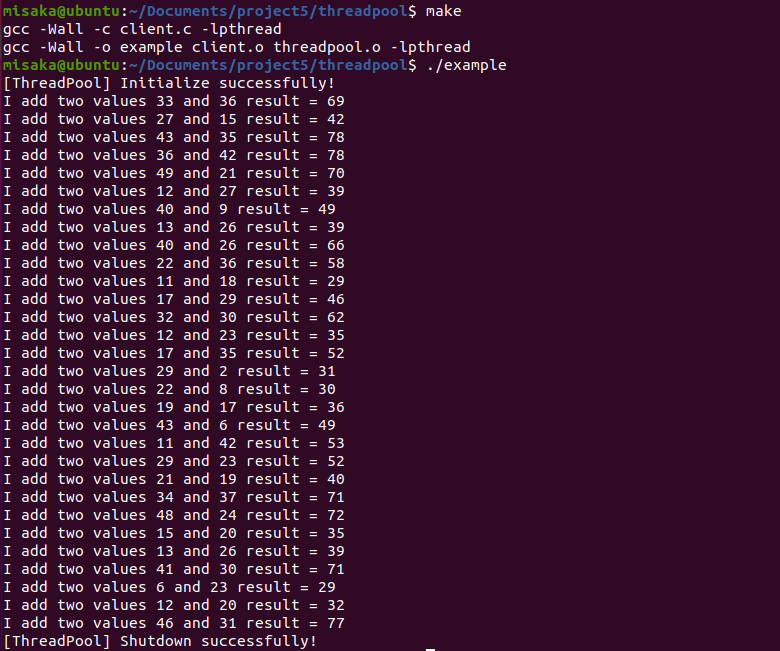
\includegraphics[width=400pt]{1.png}
    \caption{Thread Pool}
    \label{3}
\end{figure}


\section{The Producer–Consumer Problem}

In this project, you will design a programming solution to the bounded-buffer problem using the producer and consumer processes shown in Figures 5.9 and 5.10. The solution presented in Section 7.1.1 uses three semaphores: empty and full, which count the number of empty and full slots in the buffer, and mutex, which is a binary (or mutual exclusion) semaphore that protects the actual insertion or removal of items in the buffer. For this project, you will use standard counting semaphores for empty and full and a mutex lock, rather than a binary semaphore, to represent mutex. The producer and consumer—running as separate threads—will move items to and from a buffer that is synchronized with the empty, full, and mutex structures. You can solve this problem using either Pthreads or the Windows API.



\textbf{Design:} My design for this task is shown as follows:

\begin{itemize}
    \item Semaphore \texttt{empty} and \texttt{full} is used to track the items in the buffer. \texttt{empty} represents the number of empty units in the buffer. \texttt{full} represents the number of full units in the buffer.
    
    \item The buffer is implemented using a circular queue.
    
    \item The producer will produce an item after a random time (from 0 to 4 seconds). The consumer will consume an item after a random time (from 0 to 4 seconds). 
    
    \item The whole program will run for \textbf{time\_all} seconds. There will be \textbf{producer\_all} producer and \textbf{consumer\_all} consumer.
\end{itemize}

The code of \texttt{buffer.c} is shown as follows.

\begin{lstlisting}[language = c ]
#include "buffer.h"

buffer_item buffer[max_buf + 1];
int head, tail;

int insert_item(buffer_item item) {
    if (head == (tail + 1) % (max_buf + 1)) return -1; // buffer is full
    tail = (tail + 1) % (max_buf + 1);
    buffer[tail] = item;
    return 0;
}

int remove_item(buffer_item *item) {
    if (head == tail) return -1;
    head = (head + 1) % (max_buf + 1);
    *item = buffer[head];
    return 0;
}

void initial_buffer() {
    head = 0;
    tail = 0;
}
\end{lstlisting}


The code of \texttt{producer-consumer.c} is shown as follows.
\begin{lstlisting}[language = c ]
#include <stdio.h>
#include <stdlib.h>
#include <pthread.h>
#include <semaphore.h>
#include <unistd.h>
#include "buffer.h"


int running = 0; // 0 -> running; 1 -> not running;

pthread_mutex_t mutex;
sem_t empty;
sem_t full;


void *producer(void *arg) {
    buffer_item item;

    while (1) {
        sleep(rand() % 5);
        sem_wait(&empty);
        pthread_mutex_lock(&mutex);

        if (running == 1) break;
        item = rand();
        if (insert_item(item) != -1) {
            fprintf(stdout, "[Producer] %d is produced.\n", item);
        } else {
            fprintf(stderr, "[Error] unreachable!\n");
			exit(1);
        }

        pthread_mutex_unlock(&mutex);
		sem_post(&full);
    }
    pthread_mutex_unlock(&mutex); // for terminating the program
	pthread_exit(0);
}

void *consumer(void *arg) {
    buffer_item item;
    
    while (1) {
        sleep(rand() % 5);
        sem_wait(&full);
        pthread_mutex_lock(&mutex);

        if (running == 1) break;
        if (remove_item(&item) != -1) {
            fprintf(stdout, "[Consumer] %d is consumed.\n", item);
        } else {
            fprintf(stderr, "[Error] unreachable!\n");
			exit(1);
        }

        pthread_mutex_unlock(&mutex);
		sem_post(&empty);
    }
    pthread_mutex_unlock(&mutex); // for terminating the program
	pthread_exit(0);
}

int main(int argc, char *argv[]) {
    pthread_t *producer_thread, *consumer_thread;
    
    if (argc != 4) {
        fprintf(stderr, "[Error] Input should be like 'producer-consumer 10 5 5'.\n");
		exit(1);
    }

    int time_all = atoi(argv[1]);
    int producer_all = atoi(argv[2]);
    int consumer_all = atoi(argv[3]);

    
    initial_buffer();
    pthread_mutex_init(&mutex, NULL);
    sem_init(&empty, 0, max_buf);
    sem_init(&full, 0, 0);

    producer_thread = (pthread_t *) malloc (sizeof(pthread_t) * producer_all);
    consumer_thread = (pthread_t *) malloc (sizeof(pthread_t) * consumer_all);

    for (int i = 0; i < producer_all; i++)
		pthread_create(&producer_thread[i], NULL, &producer, NULL);
	for (int i = 0; i < consumer_all; i++)
		pthread_create(&consumer_thread[i], NULL, &consumer, NULL);

    sleep(time_all);

    running = 1;

    for (int i = 0; i < producer_all; i++)
		sem_post(&empty);
	for (int i = 0; i < consumer_all; i++)
		sem_post(&full);
    
    for (int i = 0; i < producer_all; i++)
		pthread_join(producer_thread[i], NULL);
	for (int i = 0; i < consumer_all; i++)
		pthread_join(consumer_thread[i], NULL);

    sem_destroy(&empty);
    sem_destroy(&full);
    pthread_mutex_destroy(&mutex);

    free(producer_thread);
    free(consumer_thread);
    return 0;
}
\end{lstlisting}

Makefile for producer consumer Problem is shown as follow.
\begin{lstlisting}
CC=gcc
CFLAGS=-Wall
PTHREADS=-lpthread

all: producer-consumer.o buffer.o
	$(CC) $(CFLAGS) -o producer-consumer buffer.o producer-consumer.o $(PTHREADS)

buffer.o: buffer.c
	$(CC) $(CFLAGS) -c buffer.c $(PTHREADS)

producer-consumer.o: producer-consumer.c
	$(CC) $(CFLAGS) -c producer-consumer.c $(PTHREADS)

clean:
	rm -rf *.o
	rm -rf producer-consumer
\end{lstlisting}


The execution result is shown as follow.
\begin{figure}[H]
    \centering
    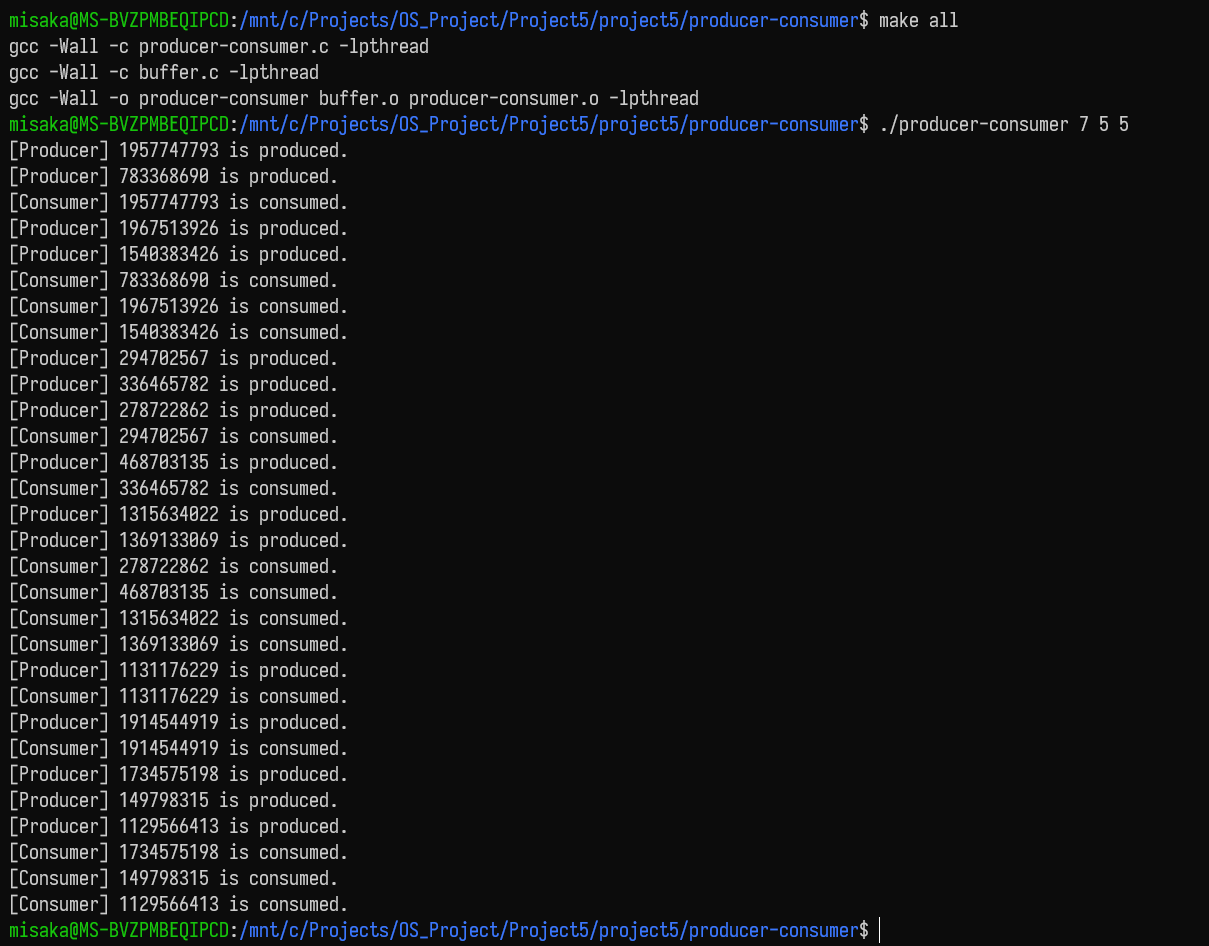
\includegraphics[width=400pt]{2.png}
    \caption{Producer Consumer Problem}
    \label{3}
\end{figure}

\end{document}